%% Document created 26 April 2022 automatically 
%% from /Users/massimosotgia/Desktop/uni_at_DIFI/Lab2/setup.py 

%% Copyright (C) Mattia Sotgia et al. 2022
%% Using class revtex4-2.cls
%                                       
%                                       
%██       █████  ██████         ██████  
%██      ██   ██ ██   ██             ██ 
%██      ███████ ██████          █████  
%██      ██   ██ ██   ██        ██      
%███████ ██   ██ ██████  ██     ███████ 
%                                       
%                                       
\documentclass[
    prl,
    % preprint,
    % linenumbers,
    % tightlines,
    reprint, 
    superscriptaddress, 
    altaffilletter, 
    amsmath, 
    amssymb, 
    a4paper,
    varvw]{revtex4-2}

\usepackage[top=1.75cm,bottom=2.5cm,left=1.5cm,right=1.5cm]{geometry}

\usepackage[utf8]{inputenc}
\usepackage[T1]{fontenc}

\usepackage[italian]{babel}

%% revtex4-2 bug-fix
\def\andname{e}
%--------------------
\makeatletter
\let\it@comma@def\active@comma
\makeatother

\usepackage{txfonts}
\usepackage{graphicx}% Include figure files
\graphicspath{{../fig/}}

\usepackage{dcolumn}% Align table columns on decimal point
\usepackage{bm}% bold math
% \usepackage[
%     % bookmarksopen=true, 
%     % citebordercolor={0 1 0}, 
%     % linkbordercolor={1 0 0}, 
%     % urlbordercolor={0 1 1}
% ]{hyperref}% add hypertext capabilities

\usepackage{physics}

\usepackage{fancyhdr}
\pagestyle{fancy}
\fancyhf{}
\def\twodigits#1{\ifnum#1<10 0\fi\the#1}

%-----------------------------------------------------------------------------------------------

\usepackage{background}
\SetBgColor{gray}
\SetBgAngle{90}
\SetBgScale{2}
\SetBgVshift{0.27\textwidth}

\usepackage[american resistors]{circuitikz}
\usepackage{listings}
\lstset{
  basicstyle=\fontsize{5}{6}\selectfont\ttfamily,
  % backgroundcolor=\color{white},   % choose the background color
  % basicstyle=\footnotesize,        % the size of the fonts that are used for the code
  breakatwhitespace=false,         % sets if automatic breaks should only happen at whitespace
  breaklines=true,                 % sets automatic line breaking
  captionpos=b,                    % sets the caption-position to bottom
  % commentstyle=\color{mygreen},    % comment style
  deletekeywords={...},            % if you want to delete keywords from the given language
  escapeinside={\%*}{*)},          % if you want to add LaTeX within your code
  % extendedchars=true,              % lets you use non-ASCII characters; for 8-bits encodings only, does not work with UTF-8
  % firstnumber=1000,                % start line enumeration with line 1000
  % frame=single,                    % adds a frame around the code
  % keepspaces=true,                 % keeps spaces in text, useful for keeping indentation of code (possibly needs columns=flexible). 
  % keywordstyle=\color{blue},       % keyword style
  % numbers=left,                    % where to put the line-numbers; possible values are (none, left, right)
  % numbersep=5pt,                   % how far the line-numbers are from the code
  numberstyle=\tiny\color{gray}, % the style that is used for the line-numbers
  % rulecolor=\color{black},         % if not set, the frame-color may be changed on line-breaks within not-black text (e.g. comments (green here))
  showspaces=false,                % show spaces everywhere adding particular underscores; it overrides 'showstringspaces'
  showstringspaces=false,          % underline spaces within strings only
  showtabs=false,                  % show tabs within strings adding particular underscores
  stepnumber=2,                    % the step between two line-numbers. If it's 1, each line will be numbered
  % stringstyle=\color{mymauve},     % string literal style
  tabsize=2,                       % sets default tabsize to 2 spaces
}

%% Define ref types
\newcommand{\reftab}[1]{Tabella {\ref{#1}}}%
\newcommand{\reffig}[1]{Figura {\ref{#1}}}%
\newcommand{\refeqn}[1]{({\ref{#1}})}%
\newcommand{\ChiSqr}{$\chi^2$\space}
\newcommand{\ChiNdf}{$\chi^2/\text{ndf}$}
\newcommand{\cernroot}{\texttt{root}}
\newcommand{\treSigma}{$3\sigma$}
\newcommand{\stdErr}[1]{$\varepsilon_{#1}$}
\newcommand{\mstdErr}[1]{\varepsilon_{#1}}
%% PAPER ONLY custom Macros

\usepackage{chemformula}
\usepackage{subfig}
\sisetup{
    % separate-uncertainty=true,
    % per-mode=symbol,
    round-mode=uncertainty,
    % exponent-mode = scientific
}

\setcounter{secnumdepth}{2}

\fancyfoot[C]{
    \the\year\twodigits\month\twodigits\day/7-\thepage
}
\fancyhead[C]{RELAZIONE DI LABORATORIO \textbf{
    N. 4 % ! <== CAMBIARE (Nessuna rel. -> 00)
    } (\the\year)
}

\begin{document}

\title{Misura della densità di portatori di carica su sonda tramite effetto Hall
}
\thanks{Esperienza n. 7
}

\author{Francesco Polleri}
\email{s5025011@studenti.unige.it}
\author{Mattia Sotgia}
\email{s4942225@studenti.unige.it}
\collaboration{Gruppo A1}
\affiliation{Dipartimento di Fisica, Università degli Studi di Genova, I-16146 Genova, Italia}

% \author{Michele Giorgi}
% \author{Lorenzo Lucentini}
% \collaboration{Gruppo C6}
% \affiliation{Dipartimento di Fisica, Università degli Studi di Genova, I-16146 Genova, Italia}


\date{presa dati
    11--12 maggio 2022, consegnata in data 
    \today
}

\begin{abstract}
    L'effetto Hall si verifica quando delle cariche transitano attraverso una corrente $i$ che è perpendicolare ad un campo magnetico $B$, tali per cui si viene a creare una tensione lungo il terzo asse ortogonale. Questa tensione è direttamente proporzionale a $i$ e $B$, ed inversamente proporzionale alla carica dei portatori e alla loro densità volumica $\eta$.
    Si vuole misurare la densità di portatori di carica di una sonda di bismuto \ch{^{83}Bi} realizzata per deposizione su film. Questa sonda è inserita nel traferro di un circuito magnetico, dove è sottoposta ad un campo $B_t$. La tensione $V_H$ è misurata direttamente sulla sonda, ottenendo quindi una stima della densità volumica di portatori $\eta$.
\end{abstract}


\maketitle
\thispagestyle{fancy}
% Rimuovere per consegna
\SetBgContents{
    laboratorio2: e7 [non per la consegna] \today % ! Note di versione
}

%%%% CORPO DEL TESTO
%%%% CORPO DEL TESTO

\section{Introduzione}

Il passaggio di corrente attraverso un sottile strato conduttore comporta la presenza di una densità di corrente, attraverso il materiale stesso, $\vec{J}=nq\vec{v}_d$, dove $\vec{v}_d$ è la velocità di drift (o di spostamento) dei portatori di carica, e $\eta$ indica la densità di portatori di carica che contribuiscono alla corrente, per unità di volume, misurata in \si{\per\cubic\metre}. Sottoponendo la lamina conduttrice ad un campo magnetico sufficientemente uniforme \footnote{Il campo magnetico deve essere posto ortogonalmente alla densità di corrente $\vec{J}$, evitando di dover effettuare anche misurazioni dell'angolo $\alpha$ di orientamento di $\vec{B}$ rispetto a $\vec{J}$.} otteniamo che le cariche saranno quindi sottoposte ad una forza di Lorentz \begin{equation}
    \vec{F}_m = q\vec{v}_d \times \vec{B} = qv_dB\hat{u}_H,\label{eq:lorentz_F_m}
\end{equation} che avrà come risultato diretto lo spostamento dei portatori di carica $q$ nella direzione $\hat{u}_H$. Considerando un materiale conduttore come composto da cariche $q$ (portatori di corrente) immersi in una distribuzione che possiamo considerare uniforme (secondo la fisica classica) di cariche $-q$ \footnote{Stiamo considerando il valore di $q$ in termini assoluti, non ponendoci quindi problemi sul segno dei portatori di un conduttore. Un conduttore è però elettricamente neutro, quindi a dei portatori di carica $q$ devono corrispondere delle cariche $-q$ che bilancino complessivamente elettricamente la carica. }, possiamo allora osservare che dopo un certo tempo \footnote{Definiamo questo tempo \emph{tempo caratteristico}, e osserviamo che è sufficientemente piccolo da poter considerare questo processo praticamente istantaneo} si formerà un campo elettrico $\vec{E}_H = \vec{F}_H/q$ in direzione ortogonale a $\vec{J}$ e $\vec{B}$, che comporterà quindi l'esistenza di una differenza di potenziale agli estremi della lamina definita come \begin{equation}
    V_H = \frac{i}{ew}\frac{1}{\eta}B,
\end{equation} dove $w$ indica lo spessore della lamina che utilizziamo, che comunque nel nostro apparato sperimentale riusciamo ad avere molto inferiore alle altre dimensioni della sonda utilizzata, e dove $i=JA$ indica il flusso della densità di corrente, ovvero la corrente attraverso una sezione $A$. L'effetto misurato è noto come effetto Hall \cite{Hall_1897}. Misurando la tensione che si viene a creare sulla lamina, possiamo ottenere quindi una misura efficace della densità di portatori in funzione delle altre variabili del nostro setup. 

I portatori di carica di un qualsiasi materiale classico sono elettroni, di carica $e=\SI{1.602176634e-19}{\coulomb}$ \footnote{valore esatto, fonte BIPM, \emph{defining constants}: \url{https://www.bipm.org/en/measurement-units/si-defining-constants}, anche in \cite{Newell_2018}}. 

\section{Metodo sperimentale}
La misura dei portatori di carica viene effettuata utilizzando una sonda di \ch{Bi} metallico costituita da un film sottile depositato su una lamina isolante. Il metodo di deposizione ci permette infatti di avere uno spessore $w$ della lamina piuttosto basso, permettendoci quindi di stabilire in modo univoco quale è la direzione perpendicolare rispetto al piano della sonda, e individuare quindi un sistema destrorso $xyz$ come in figura \ref{fig:sonda.rotated}. Il sistema così individuato può essere utilizzato come riferimento per tutti i calcoli che verranno svolti.

La corrente infatti scorre nel verso negativo di $\hat{e}_1$, che invece è rivolto nella direzione di $\vec{J}$ coerentemente alla direzione della velocità di drift $v_e$ degli elettroni. Tale corrente viene controllata attraverso un generatore calibrato per avere in uscita una corrente costante inferiore a \SI{10}{\milli\ampere} per permettere alla sonda di lavorare in condizioni di dissipazione dell'energia controllate e per avere inoltre fluttuazioni rispetto al valore medio molto inferiori a quelle che si avrebbero collegando semplicemente il generatore da banco, che essendo costruito per un utilizzo generico può non essere la scelta migliore per l'uso specifico di cui necessitiamo. Il generatore di corrente infatti permette di avere un valore di corrente in uscita pari a $\SI{1.7242(300)e-3}{\ampere\per\volt}\times\qty(V_--V_+)$, dove $V_--V_+$ è la differenza di tensione fornita in ingresso al generatore di corrente (per la caratterizzazione del generatore di corrente vedere l'appendice \ref{sec:appendix_current_gen}). Della tensione che forniamo al generatore facciamo una serie di misure insieme alla presa dati e dopo una trattazione di tipo statistico degli errori, troviamo un'incertezza sulla tensione di \SI{2.6}{\milli\volt} e quindi una deviazione standard sulla corrente inferiore a 18 ppt \footnote{Otteniamo una corrente di \SI[separate-uncertainty=true]{8.619(150)}{\milli\ampere}}. 

Ciò che adesso ci manca è il campo magnetico a cui sottoponiamo la cariche presenti nella sonda. Per creare tale campo $B$ sono possibili diverse opzioni e noi abbiamo scelto quella di utilizzare un elettromagnete (vedi \reffig{??}). Tale strumento ci permette infatti di creare un campo magnetico con un modulo sufficientemente elevato per il tipo di misure che vogliamo effettuare, cosa che una semplice bobina non sarebbe stata in grado di fare e inoltre, se nell'elettromagnete è presente un traferro, in quel punto il campo $B$ è uniforme e sono trascurabii gli effetti di bordo. Altra cosa importante è che il campo è anche facilmente controllabile dalle correnti che scorrono nelle bobine avvolte intorno ai suoi bracci. Se il materiale con cui l'elettromagnete è stato realizzato è ferro dolce allora il suo ciclo di isteresi sarà stretto per cui possiamo approssimare che per valori non troppo elevati di corrente la risposta del campo magnetico sia lineare. Per evitare possibili problemi legati alla magnetizzazione residua decidiamo di fare la presa dati fornendo alle bobine dell'elettromagnete valori di corrente sempre decrescenti, che partendo da un determinato valore, scendano sino ad avere corrente nulla e poi crescano di nuovo ma nel verso opposto. 
Dalla misura delle dimensioni dell'elettromagnete possiamo risalire, attraverso la legge di Hopkinson, all'equazione che ci permette di calcolare $B$ nel traferro. Siccome l'elettromagnete è costituito da due bobine e la corrente che circola in esse è tale che il flusso dei campi magnetici prodotti si sommi nel braccio dell'elettromagnete dove è presente il traferro e siccome la sezione del braccio del traferro è doppia rispetto alla sezione del braccio delle bobine, possiamo calcolare $B$ come se l'elettromagnete fosse costituito da una sola bobina e poi moltiplicare tale valore per due. Per la legge di Hopkinson sappaimo che  $\Phi\cdot R=N\cdot I$ dove $R$ rappresenta la riluttanza complessiva dell'elettromagnete, costituita dalla somma della riluttanza del traferro ($R_{t}$) e del ferro ($R_{f}$).
$R_{t}=\frac{l_{t}}{\mu_{0}S_{t}}$ mentre $R_{f}=\frac{l_{f}}{\mu_{0}\mu_{r}S_{f}}$ dove $l_{t}$ rappresenta lo spessore del traferro, $l_{f}$ la lunghezza dell'anello dell'elettromagnete tolto lo spessore del traferro, $S_{f}$ la sezione del braccio del


\begin{figure}
    \subfloat[][]{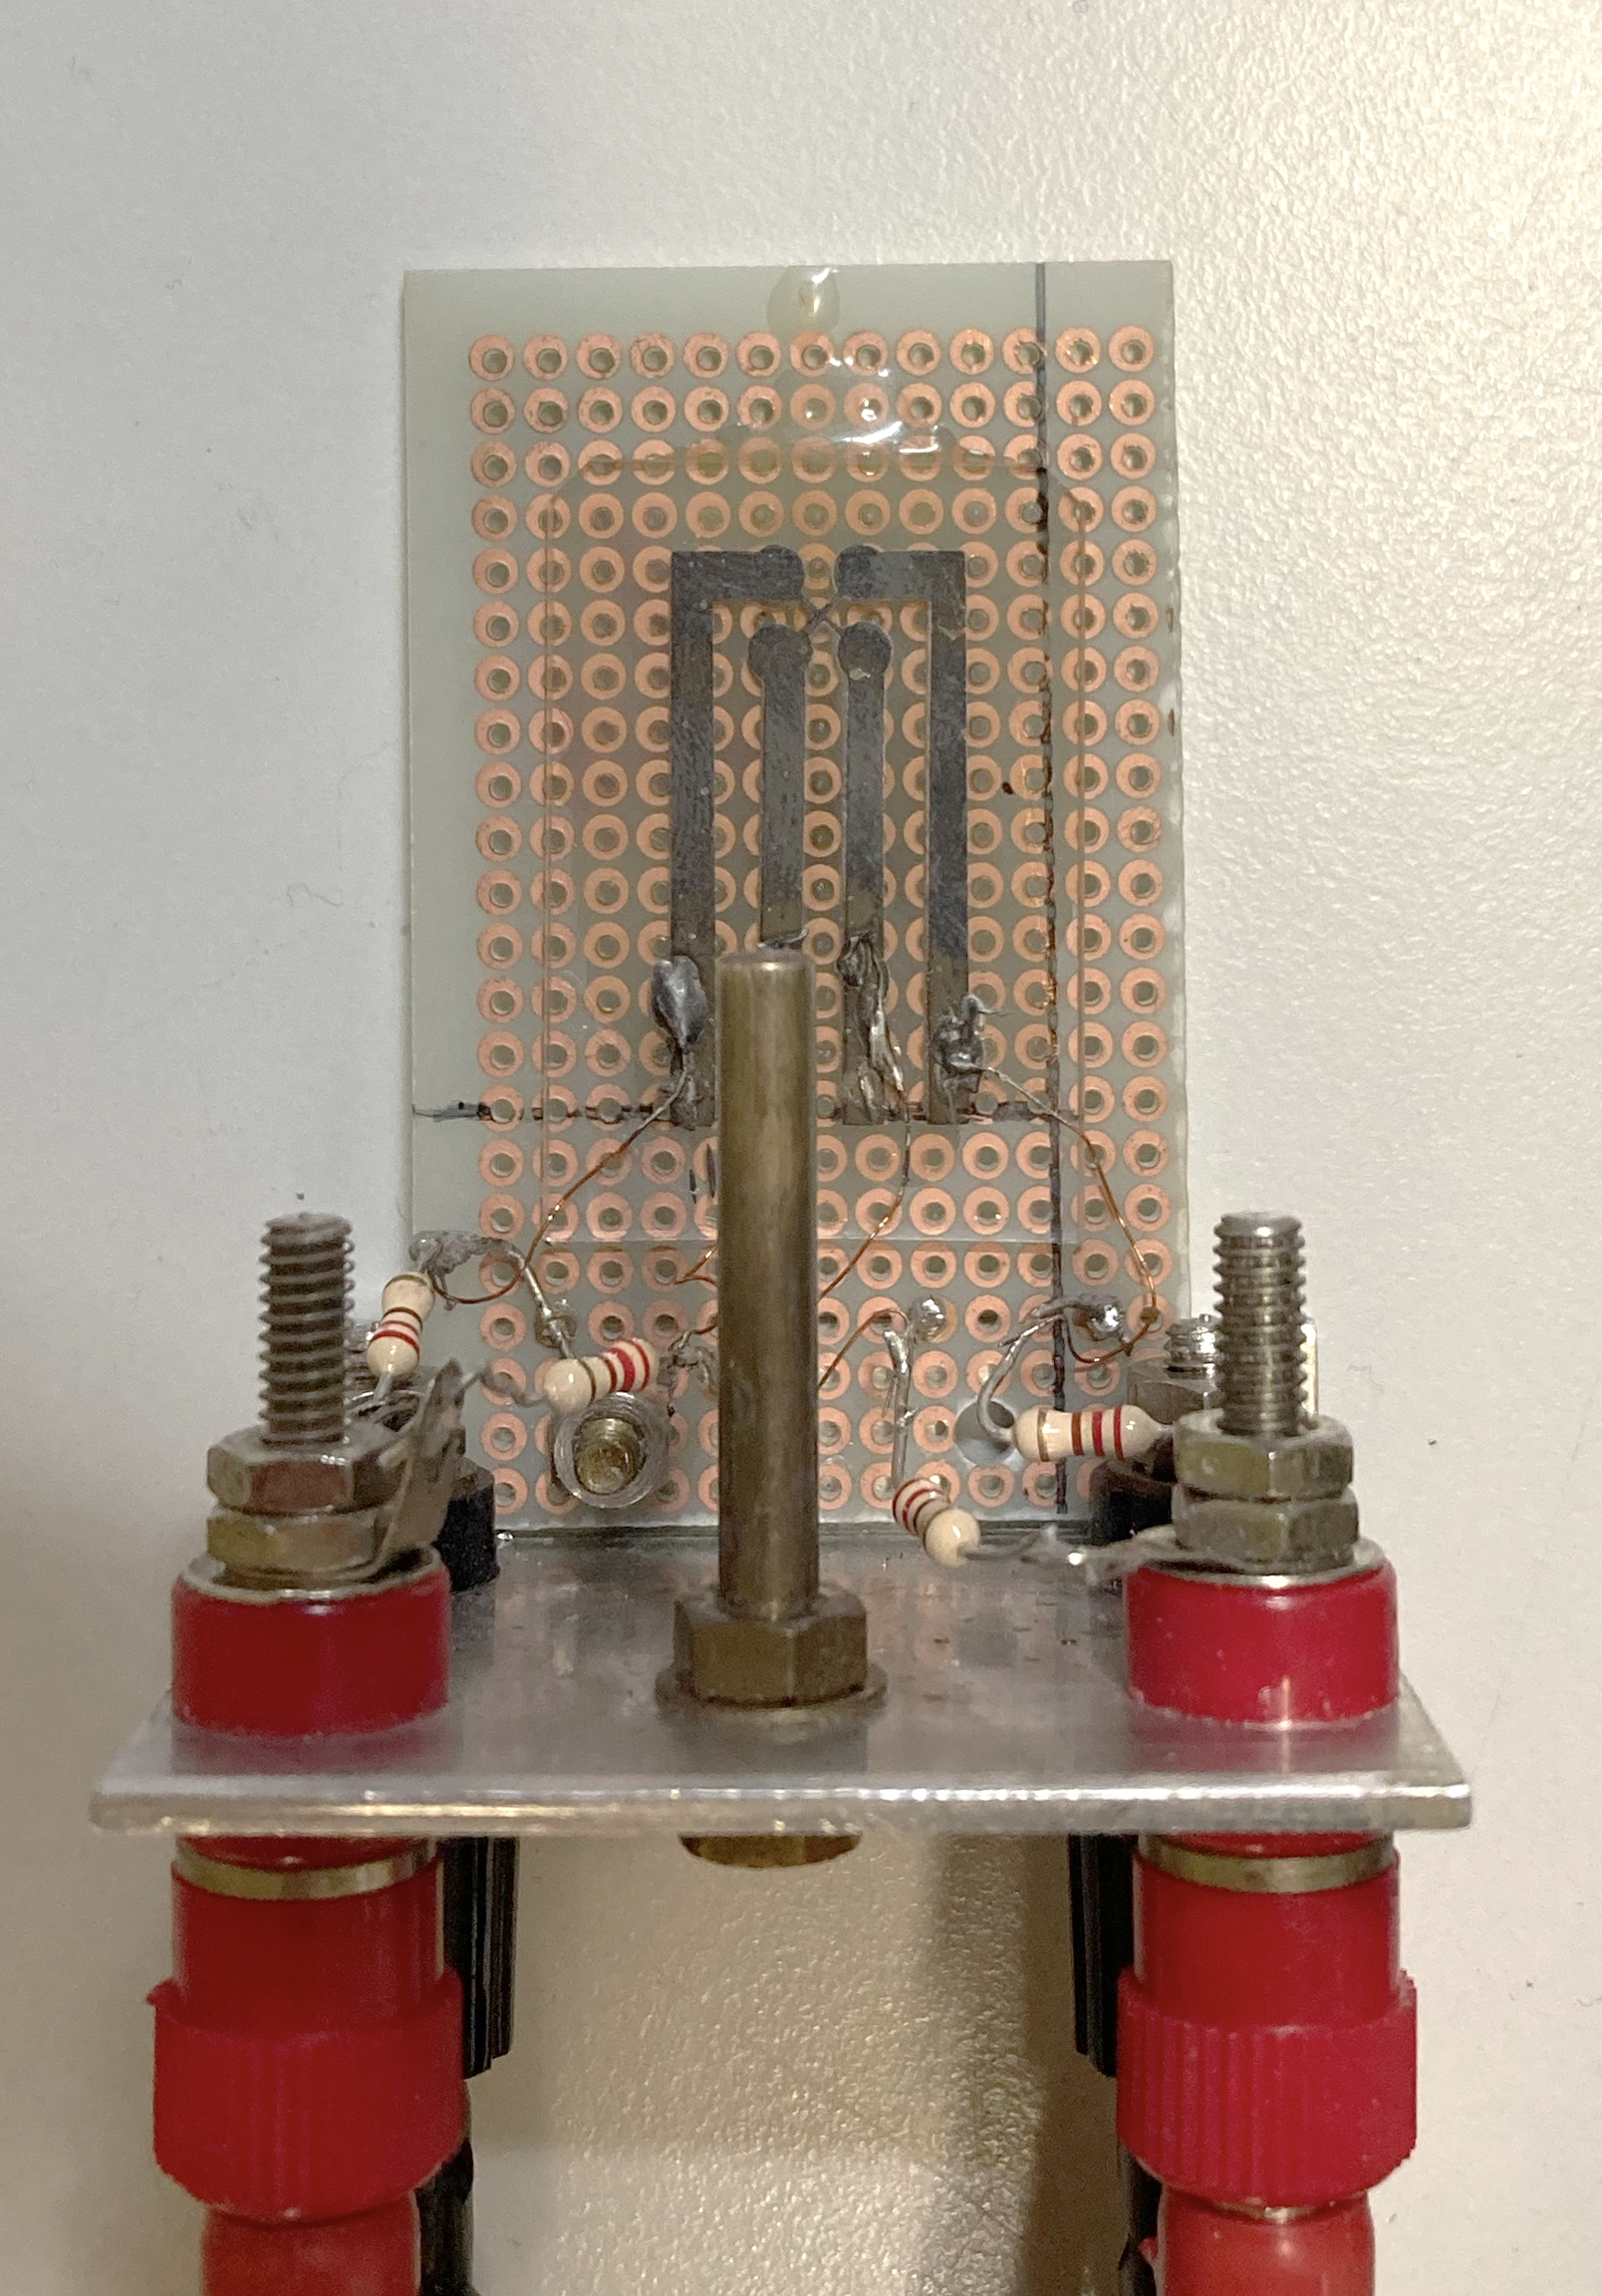
\includegraphics[width=0.3\linewidth]{sonda.IMG_0233.png}\label{fig:sonda.IMG}}\hspace{5mm}
    \subfloat[][]{
        \begin{tikzpicture}
            \draw node[inner sep=0] (0) at (-.1,0) {\includegraphics[width=3.5cm]{sonda.IMG_0233_cropped_rotated.png}};
            \draw[-latex, white] (0,.1) to (0,.5) node[above] {$\vu{e}_1$};
            \draw[-latex, white] (.1,0) to (.5,0) node[right] {$\vu{e}_3$};
            \draw[white] (0,0) node[left] {$\vu{e}_2$};
            % \filldraw[white] (0, 0) circle (0.1) 
            \draw node[white] {$\mathbf{\odot}$};
        \end{tikzpicture}
    \label{fig:sonda.rotated}}
    \caption{Dettaglio della sonda utilizzata per misurare l'effetto Hall. In (b) indichiamo anche una terna destrorsa utilizzata per considerazioni fisiche. }\label{fig:misc}
\end{figure}

% posta in un campo magnetico generato all'interno di un traferro da un elettromagnete che lavora a correnti variabili tra \SI{0.1}{\ampere} e \SI{1.3}{\ampere}. Il campo magnetico così generato risulta essere molto potente e abbastanza stabile. La sonda è poi attraversata ortogonalmente rispetto alla direzione di $\vec{B}_t$ da una corrente $i_s$. Questa corrente 


%\onecolumngrid
\appendix
\section{Caratterizzazione del generatore di corrente}\label{sec:appendix_current_gen}
In figura \reffig{??} è riportato lo schema circuitale del circuito del generatore di corrente. Tale circuito è tale per cui data una differenza di potenziale fornita al circuito come $V^{-}-V^{+}$ si ha in uscita una corrente $I_{out}=\frac{R_{2}}{R_{1}}\cdot \frac{V^{-}-V^{+}}{R_{5}}$. Siccome abbiamo previsto che la tensione che forniamo al circuito è pari a \SI{5}{\volt} e vogliamo che la corrente cha va alla sonda non superi \SI{10}{\milli\ampere} allora il fattore $\frac{R_{2}}{R_{1}}\cdot \frac{1}{R_{5}}=G_{g}$ dovrà essere almeno pari a $\frac{1}{500}$. Scegliamo quindi $R_{1}=R_{2}=\SI{1}{\kilo\ohm}$ e $R_{5}=\SI{500}{\ohm}$. Per verificare se effettivamente il fattore $G_{g}$ sia pari a $1/500$ possiamo raccogliere una serie di coppie valori di $I_{out}$ e $V^{-}-V^{+}$ e realizzare un fit \reffig{??} secondo la funzione $I_{out}=G_{g}\cdot V^{-}-V^{+}+I_{0}$ dove scegliamo come parametri di fit $G_{g}$ e $I_{0}$. Otteniamo che 
\begin{align}
    G_{g} &=\SI{1.7242(300)}{\milli\ampere \per\volt}  \\
    I_{0} &= \SI{0.0673(889)}{\ampere}.
\end{align}
Il valore teorico di $G_{g}$ è ?? \SI{}{} per cui troviamo che è compatibile con il valore ricavato dal fit e troviamo anche che il valore di $I_{0}$ è compatibile con zero, per cui possiamo dire che non c'è un offset sulla corrente che mandiamo alla sonda.
Un ulteriore test fatto è stato quello di mantenere costante il valore di $V^{-}-V^{+}$ e verificare che, cambiando il carico in uscita dal generatore, la corrente rimane sempre la stessa.
\section{Caratterizzazione dell'amplificatore operazionale per strumentazione}\label{sec:appendix_strum_opamp}
In figura \reffig{??} è riportato lo schema circuitale dell'amplificatore per strumentazione che  è caratterizzato da un guadagno complessivo dato da \begin{equation}V_{out} = G_{\text{diff}}\cdot \left(V_{\text{non-inv}}-V_{\text{inv}}\right) +  G_{\text{CM}}\cdot V_{\text{CM}} + V_{\text{offset}} \end{equation}
La parte predominante di questo guadagno è data $G_{diff}$ che è pari a $\frac{R_{d}}{R_{c}}\cdot \left(1+2\cdot \frac{R_{b}}{R_{a}}\right)$ e vogliamo che sia pari a 200. Scegliamo quindi 

% \begin{figure}
%     \centering
%     \includegraphics[width=\linewidth]{G_CM.pdf}
%     \includegraphics[width=\linewidth]{G_diff.pdf}
%     \caption{Analisi del guadagno di modo comune (a) e del guadagno differenziale (b) dell'amplificatore operazionale per strumentazione.}
% \end{figure}

\setcounter{table}{0}
\renewcommand{\thetable}{A-\Roman{table}}

%\bibliographystyle{plain}
\bibliography{references/IOP.shortcomm.CODATA2017, references/10.2307_2369245}

\end{document}
    
